\documentclass[11pt,a4paper]{article}

% ---------- Packages ----------
\usepackage[margin=2.2cm]{geometry}
\usepackage{xcolor}
\usepackage{graphicx}
\usepackage{booktabs}
\usepackage{tabularx}
\usepackage{array}
\usepackage{enumitem}
\usepackage{listings}
\usepackage{fancyhdr}
\usepackage{titlesec}
\usepackage{tikz}
\usetikzlibrary{arrows.meta,positioning,shapes.multipart,shapes.geometric,calc,fit}
\usepackage[most]{tcolorbox}
\usepackage[hidelinks]{hyperref}

% ---------- Colours ----------
\definecolor{brand}{HTML}{1F4E79}
\definecolor{brandlight}{HTML}{E8F0F8}
\definecolor{okgreen}{HTML}{1E7B4F}
\definecolor{okbg}{HTML}{E9F6EF}
\definecolor{warnorange}{HTML}{A85A00}
\definecolor{warnbg}{HTML}{FFF4E5}
\definecolor{codebg}{HTML}{F6F8FA}
\definecolor{codeframe}{HTML}{D0D7DE}
\definecolor{kw}{HTML}{8250DF}
\definecolor{str}{HTML}{0A3069}
\definecolor{cmt}{HTML}{6E7781}

% ---------- Layout ----------
\setlength{\parindent}{0pt}
\setlength{\emergencystretch}{3em}
\sloppy
\setlength{\parskip}{6pt}
\setlist{itemsep=2pt,topsep=4pt}
\titleformat{\section}{\Large\bfseries\color{brand}}{\thesection}{0.8em}{}
\titleformat{\subsection}{\large\bfseries\color{brand}}{\thesubsection}{0.8em}{}
\titleformat{\subsubsection}{\normalsize\bfseries}{\thesubsubsection}{0.8em}{}
\pagestyle{fancy}
\fancyhf{}
\fancyhead[L]{\small\color{brand}FinCore --- Phase 1 Explained}
\fancyhead[R]{\small\color{brand}\leftmark}
\fancyfoot[C]{\small\thepage}
\renewcommand{\headrulewidth}{0.4pt}

% ---------- Helpers ----------
\newcommand{\code}[1]{\texttt{\detokenize{#1}}}

\newtcolorbox{whybox}[1][Why?]{enhanced,breakable,colback=brandlight,colframe=brand,
  fonttitle=\bfseries,title=#1,arc=2pt,boxrule=0.6pt,left=6pt,right=6pt}
\newtcolorbox{simplebox}[1][In simple words]{enhanced,breakable,colback=okbg,colframe=okgreen,
  fonttitle=\bfseries,title=#1,arc=2pt,boxrule=0.6pt,left=6pt,right=6pt}
\newtcolorbox{warnbox}[1][Watch out]{enhanced,breakable,colback=warnbg,colframe=warnorange,
  fonttitle=\bfseries,title=#1,arc=2pt,boxrule=0.6pt,left=6pt,right=6pt}
\newtcolorbox{interviewbox}[1][Interview angle]{enhanced,breakable,colback=white,colframe=kw,
  fonttitle=\bfseries,title=#1,arc=2pt,boxrule=0.6pt,left=6pt,right=6pt}

\lstdefinestyle{java}{
  language=Java,
  basicstyle=\ttfamily\footnotesize,
  keywordstyle=\color{kw}\bfseries,
  stringstyle=\color{str},
  commentstyle=\color{cmt}\itshape,
  backgroundcolor=\color{codebg},
  frame=single, rulecolor=\color{codeframe},
  breaklines=true, breakatwhitespace=false,
  showstringspaces=false, columns=fullflexible, keepspaces=true,
  xleftmargin=4pt, xrightmargin=4pt, aboveskip=8pt, belowskip=8pt,
  morekeywords={record,var},
  moredelim=[s][\color{okgreen}]{@}{\ }
}
\lstdefinestyle{plain}{
  language={},
  basicstyle=\ttfamily\footnotesize,
  backgroundcolor=\color{codebg},
  frame=single, rulecolor=\color{codeframe},
  breaklines=true, columns=fullflexible, keepspaces=true,
  showstringspaces=false, xleftmargin=4pt, xrightmargin=4pt
}
\lstset{style=java}

\hypersetup{pdftitle={FinCore - Phase 1 Explained},pdfauthor={Piyush Kumar Sharma}}

\begin{document}

% ================= TITLE =================
\begin{titlepage}
\centering
\vspace*{3cm}
{\Huge\bfseries\color{brand} FinCore\par}
\vspace{0.4cm}
{\Large Secure Digital Wallet \& Payments REST API\par}
\vspace{1.2cm}
{\LARGE\bfseries Phase 1 Explained\par}
\vspace{0.3cm}
{\large What was built, why it was built that way, and how it works\\ --- in simple terms\par}
\vspace{2cm}
\begin{tcolorbox}[colback=brandlight,colframe=brand,width=0.8\textwidth,arc=2pt]
\centering
\begin{tabular}{rl}
\textbf{Author} & Piyush Kumar Sharma, B.Tech ECE, NIT Silchar \\
\textbf{Repository} & \url{https://github.com/piyush-nfx/fincore} \\
\textbf{Commit} & \code{8d0a2bd} on \code{main} (old CLI kept as tag \code{v1-cli}) \\
\textbf{Stack} & Java 25, Spring Boot 4.1, Spring Data JPA, MySQL 8 \\
\textbf{Status} & Phase 1 done: 11/11 unit tests, 16/16 Postman checks \\
\end{tabular}
\end{tcolorbox}
\vfill
{\small How to read this: every section follows the same pattern ---
\textbf{What} we built, \textbf{Why} we chose it, and \textbf{How} it works.
Coloured boxes give plain-language summaries, warnings, and interview tips.\par}
\end{titlepage}

\tableofcontents
\newpage

% =====================================================================
\section{The Big Picture}
% =====================================================================

\subsection{What is FinCore?}
FinCore is the \emph{backend} of a digital wallet, like the server behind Paytm or PhonePe
(there is no app or website, only the server). Other programs talk to it over HTTP by sending
JSON. It can:

\begin{itemize}
  \item register users,
  \item create wallets for them (each wallet holds money in one currency, e.g.\ INR),
  \item deposit money into a wallet,
  \item transfer money from one wallet to another (peer-to-peer, ``P2P''),
  \item keep a permanent record (a \emph{ledger}) of every money movement.
\end{itemize}

The name is \textbf{Fin}ance + \textbf{Core}, from ``core banking system'': the central
software of a bank that holds accounts and moves money.

\subsection{Why rebuild CryptoVault?}
FinCore replaces your older project, \textbf{CryptoVault}: a command-line Java program that
simulated a wallet using an \code{ArrayList} in memory and saved data to a text file.
That design is fine for learning OOP, but it breaks down for a real money system:

\begin{center}
\begin{tabularx}{\textwidth}{>{\bfseries}l X X}
\toprule
Problem & CryptoVault (v1) & FinCore (v2) \\
\midrule
Many users at once & One person at a keyboard; an \code{ArrayList} is not safe if two threads change it together. & A web server handles many requests in parallel; the database + optimistic locking keep balances correct. \\
Durability & If the program crashes mid-write, the text file can be half-written or lost. & MySQL transactions: a change is either fully saved or not saved at all. \\
Who are you? & No login; whoever runs the program controls everything. & Users with BCrypt-hashed passwords now; JWT login and ownership checks in Phase 2. \\
History & A log file that can be edited. & An append-only ledger table that the code never updates. \\
Access & Only on your machine. & An HTTP API any client can call; deployable to the cloud (Phase 4). \\
\bottomrule
\end{tabularx}
\end{center}

\begin{simplebox}
CryptoVault was a notebook on your desk. FinCore is a bank vault with a guard, a camera, and
a logbook nobody can erase.
\end{simplebox}

\subsection{The four phases}
\begin{center}
\begin{tabularx}{\textwidth}{>{\bfseries}l X l}
\toprule
Phase & Goal & Status \\
\midrule
1 --- Core API & Users, wallets, deposits, safe transfers, error handling, tests & \textcolor{okgreen}{\textbf{Done}} \\
2 --- Security & Login, JWT tokens, ``you can only touch your own wallet'', admin role & Next \\
3 --- Production features & Automatic retry on conflicts, mandatory idempotency key, paginated history, Swagger & Planned \\
4 --- Ship it & Concurrency test, Docker, deploy online, README & Planned \\
\bottomrule
\end{tabularx}
\end{center}

This document covers \textbf{everything done up to the end of Phase 1}, including setup,
design decisions, every class, the tests, the Git history, and the problems we hit on the way.

% =====================================================================
\section{Setting Up the Project}
% =====================================================================

\subsection{What we found on your machine}
Before writing code, I checked which tools were installed, so the plan would match reality:

\begin{center}
\begin{tabularx}{\textwidth}{l l X}
\toprule
Tool & Found? & What it means \\
\midrule
Java (JDK) & Yes, 25.0.3 & We can use the newest Java. \\
Maven & No & Maven builds Java projects. We use the \emph{Maven Wrapper} (\code{mvnw.cmd}) instead, which downloads the right Maven automatically. \\
MySQL & Yes, service \code{MySQL80} running & The database is ready locally. \\
Git & Yes & Version control works. \\
Docker & No & Needed only in Phase 4; you will install Docker Desktop then. \\
\bottomrule
\end{tabularx}
\end{center}

\subsection{The generated project, and two fixes}
You generated the starter project on \url{https://start.spring.io}. When I opened it I found two
things that did not match the plan:

\begin{enumerate}
  \item \textbf{Wrong database driver.} The \code{pom.xml} contained \code{mssql-jdbc}, which is the
  driver for \emph{Microsoft SQL Server}, not MySQL. The app would never have connected to your
  database. I replaced it with \code{com.mysql:mysql-connector-j}.
  \item \textbf{Spring Boot 4.1.2 instead of 3.x.} Your brief said 3.x, but the generator picked 4.1.2.
  We decided to \textbf{stay on 4.1}.
\end{enumerate}

\begin{whybox}[Why stay on Spring Boot 4.1?]
Free (open-source) support for Spring Boot 3.5 ended in mid-2026, so 4.x is the line that still
gets security fixes. For this project the code is almost identical. The differences you will see
compared with 3.x tutorials are small: the web starter is called \code{spring-boot-starter-webmvc},
it uses Spring Framework 7 / Hibernate 7 / Jackson 3, and HTTP status 422 is called
\code{UNPROCESSABLE_CONTENT}. Saying ``I used the current supported version and handled the
migration differences'' is a good interview point.
\end{whybox}

\subsection{The dependencies, one by one}
A \emph{dependency} is a library your project uses. Maven downloads them based on
\code{pom.xml}.

\begin{center}
\begin{tabularx}{\textwidth}{>{\ttfamily}l X}
\toprule
\normalfont\bfseries Dependency & \bfseries What it gives us \\
\midrule
spring-boot-starter-webmvc & An embedded web server (Tomcat) and the tools to write REST controllers. JSON conversion via Jackson. \\
spring-boot-starter-data-jpa & JPA/Hibernate: map Java classes to tables, and Spring Data repositories so we do not write SQL for basic queries. \\
mysql-connector-j & The driver that lets Java talk to MySQL. \\
spring-boot-starter-security & Spring Security. In Phase 1 we use only its BCrypt password hasher and open all endpoints; Phase 2 locks them down. \\
spring-boot-starter-validation & Annotations like \code{@NotNull}, \code{@Positive}, \code{@Email} that check incoming data automatically. \\
lombok & Generates boilerplate (getters, constructors) at compile time, e.g.\ \code{@Getter}. \\
spring-boot-devtools & Auto-restarts the app when you change code (development only). \\
\textrm{*-test starters} & JUnit 5, Mockito, AssertJ and Spring test helpers. \\
\bottomrule
\end{tabularx}
\end{center}

% =====================================================================
\section{Configuration and Secrets}
% =====================================================================

\subsection{What: \code{application.properties}}
This file tells Spring Boot how to run. Here is the final version, explained line by line:

\begin{lstlisting}[style=plain]
spring.application.name=fincore
server.port=8083

spring.config.import=optional:file:.env[.properties]
spring.datasource.url=${DB_URL:jdbc:mysql://localhost:3306/fincore?createDatabaseIfNotExist=true}
spring.datasource.username=${DB_USERNAME:root}
spring.datasource.password=${DB_PASSWORD}

spring.jpa.hibernate.ddl-auto=update
spring.jpa.open-in-view=false
spring.jpa.show-sql=false
\end{lstlisting}

\begin{itemize}
  \item \code{server.port=8083} --- you chose this port; the app listens on \url{http://localhost:8083}.
  \item \code{spring.config.import=optional:file:.env[.properties]} --- also read settings from a file named
  \code{.env} in the project folder. \code{optional:} means ``don't crash if it's missing''.
  \item \code{${DB_URL:...}} --- use the value of \code{DB_URL}; if it isn't set, use the default after the colon.
  \item \code{${DB_PASSWORD}} --- no default on purpose: the password must come from \code{.env} or the environment.
  \item \code{ddl-auto=update} --- Hibernate creates/adjusts tables to match the entity classes at startup.
  Handy while developing; in production we switch to \code{validate} (check, never change).
  \item \code{open-in-view=false} --- explained below.
\end{itemize}

\subsection{Why secrets live in \code{.env}}
At one point you had written the real MySQL password directly into \code{application.properties}.
That file is committed to GitHub, and \textbf{anything pushed to a public repository can be copied by
anyone, even if you delete it later} (it stays in Git history). So:

\begin{itemize}
  \item the real values went into \code{.env} (project root), which is listed in \code{.gitignore}, so Git never sees it;
  \item \code{.env.example} is committed instead, with placeholder values, so others know what to fill in;
  \item before committing, I searched the staged files for the password to confirm it was not included.
\end{itemize}

\begin{simplebox}
\code{application.properties} is the recipe and is public. \code{.env} is the key to your house:
it stays in your pocket. On the cloud server (Phase 4) the same names (\code{DB_PASSWORD}, etc.)
will be set as environment variables in the hosting dashboard.
\end{simplebox}

\subsection{Why \code{open-in-view=false}}
By default Spring keeps the database session open until the HTTP response is fully written
(``Open Session In View''). That lets lazy-loaded data be fetched by accident while JSON is being
generated: hidden extra queries and database connections held for too long. Turning it off forces all
database work to happen inside the service layer's transactions, which is cleaner and easier to reason
about. That is also why we convert entities to DTOs \emph{inside} services.

\subsection{The \code{jdbc\_learning} incident (and the lesson)}
Your \code{.env} first pointed to your existing database \code{jdbc_learning}. It already had a
\code{users} table (from your JDBC practice), with an \code{address} table referencing it.
Because \code{ddl-auto=update} tries to make tables match the entities, Hibernate would \emph{add}
FinCore's columns to your old \code{users} table. When you tried to drop that table, MySQL refused
(error 3730) because \code{address.uid} is a foreign key pointing at it.

\textbf{Fix:} FinCore got its own database. \code{DB_URL} now ends in
\code{/fincore?createDatabaseIfNotExist=true}, so MySQL creates \code{fincore} on first start.

\begin{warnbox}[Lesson]
One application, one database (or schema). Sharing a database between unrelated projects
causes name clashes (two different \code{users} tables) and makes it risky to change either one.
\end{warnbox}

% =====================================================================
\section{Architecture: How the Code Is Organised}
% =====================================================================

\subsection{Layered architecture}
The code is split into layers. Each layer has one job and only talks to the layer below it.

\begin{center}
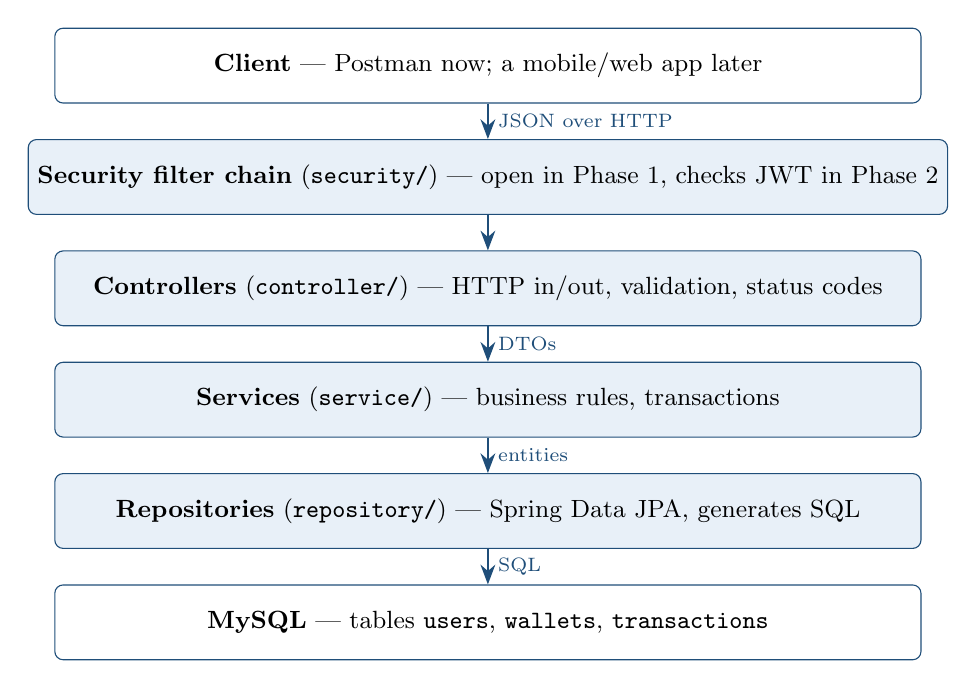
\begin{tikzpicture}[
  layer/.style={draw=brand,fill=brandlight,rounded corners=3pt,minimum width=11cm,minimum height=0.95cm,align=center,font=\small},
  arr/.style={-{Stealth[length=2.5mm]},thick,brand}]
\node[layer,fill=white] (client) {\textbf{Client} --- Postman now; a mobile/web app later};
\node[layer,below=0.45cm of client] (sec) {\textbf{Security filter chain} (\code{security/}) --- open in Phase 1, checks JWT in Phase 2};
\node[layer,below=0.45cm of sec] (ctrl) {\textbf{Controllers} (\code{controller/}) --- HTTP in/out, validation, status codes};
\node[layer,below=0.45cm of ctrl] (svc) {\textbf{Services} (\code{service/}) --- business rules, transactions};
\node[layer,below=0.45cm of svc] (repo) {\textbf{Repositories} (\code{repository/}) --- Spring Data JPA, generates SQL};
\node[layer,below=0.45cm of repo,fill=white] (db) {\textbf{MySQL} --- tables \code{users}, \code{wallets}, \code{transactions}};
\draw[arr] (client) -- node[right,font=\scriptsize]{JSON over HTTP} (sec);
\draw[arr] (sec) -- (ctrl);
\draw[arr] (ctrl) -- node[right,font=\scriptsize]{DTOs} (svc);
\draw[arr] (svc) -- node[right,font=\scriptsize]{entities} (repo);
\draw[arr] (repo) -- node[right,font=\scriptsize]{SQL} (db);
\end{tikzpicture}
\end{center}

Alongside these layers: \code{entity/} (the Java classes that map to tables), \code{dto/} (the shapes of
requests and responses), and \code{exception/} (custom errors plus one global error handler).

\begin{whybox}
\textbf{Separation of concerns.} Controllers don't know SQL; repositories don't know HTTP. You can
change one layer (e.g.\ swap MySQL for PostgreSQL, or add a GraphQL API) without rewriting the rest.
It also makes testing easy: we unit-tested \code{TransferService} by replacing the repositories with
fakes (mocks).
\end{whybox}

\subsection{Package structure}
\begin{lstlisting}[style=plain]
com.piyush.fincore
|-- FincoreApplication.java          (main method, starts Spring Boot)
|-- controller   AuthController, WalletController, TransferController
|-- service      UserService, WalletService, TransferService, FailedTransferRecorder
|-- repository   UserRepository, WalletRepository, TransactionRepository
|-- entity       User, Wallet, Transaction, Role, TransactionType, TransactionStatus
|-- dto          RegisterRequest, CreateWalletRequest, DepositRequest, TransferRequest,
|                UserResponse, WalletResponse, TransactionResponse, ErrorResponse
|-- security     SecurityConfig
`-- exception    BusinessException + 5 subclasses, GlobalExceptionHandler
\end{lstlisting}

\subsection{The journey of one request}
Here is what happens, step by step, when Postman sends a transfer:

\begin{lstlisting}[style=plain]
POST http://localhost:8083/api/transfers
Idempotency-Key: 6f1c...e2
{ "fromWalletId": 1, "toWalletId": 2, "amount": 250.50 }
\end{lstlisting}

\begin{enumerate}
  \item \textbf{Tomcat} (the embedded web server) receives the HTTP request.
  \item \textbf{Spring Security's filter chain} looks at it. In Phase 1 it lets everything through.
  \item \textbf{DispatcherServlet} (Spring's front desk) finds the method mapped to \code{POST /api/transfers}:
        \code{TransferController.transfer()}.
  \item \textbf{Jackson} converts the JSON body into a \code{TransferRequest} Java object.
  \item \textbf{Bean Validation} checks the annotations (\code{@NotNull}, \code{@Positive}, \ldots).
        If any fail, the request stops here with a 400 error.
  \item The controller checks the \code{Idempotency-Key} header length and calls \code{TransferService.transfer()}.
  \item Spring has wrapped the service in a \textbf{proxy} that \textbf{opens a database transaction}.
  \item The service loads both wallets (SQL \code{SELECT}), debits, credits, and inserts a ledger row.
  \item The method returns, so the proxy \textbf{commits}: Hibernate sends the \code{UPDATE}s and \code{INSERT}
        to MySQL, all at once.
  \item The service returns a \code{TransactionResponse}; Jackson turns it into JSON; the client gets \code{201 Created}.
  \item If \emph{anything} threw an exception in steps 8--9, the proxy \textbf{rolls back} instead, and the
        \code{GlobalExceptionHandler} turns the exception into a clean JSON error.
\end{enumerate}

% =====================================================================
\section{The Data Model (Entities)}
% =====================================================================

\subsection{The three tables}
\begin{center}
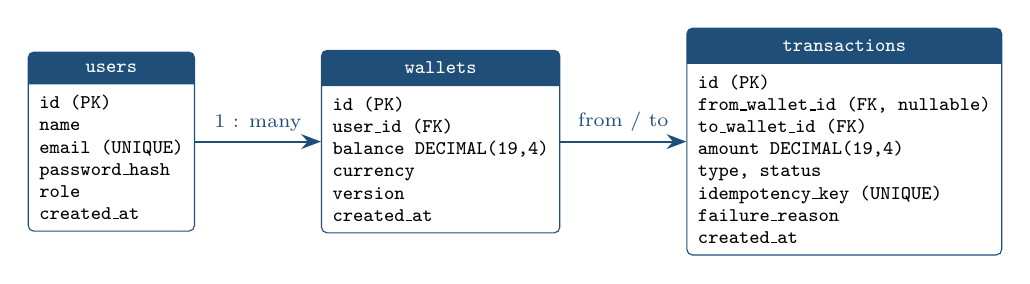
\begin{tikzpicture}[
  tbl/.style={draw=brand,rectangle split,rectangle split parts=2,rectangle split part fill={brand,white},
              align=left,font=\scriptsize\ttfamily,inner sep=4pt,rounded corners=2pt},
  rel/.style={-{Stealth[length=2.5mm]},thick,brand}]
\node[tbl] (users) {\textcolor{white}{\bfseries users}
  \nodepart{two}id (PK)\\ name\\ email (UNIQUE)\\ password\_hash\\ role\\ created\_at};
\node[tbl,right=1.6cm of users] (wallets) {\textcolor{white}{\bfseries wallets}
  \nodepart{two}id (PK)\\ user\_id (FK)\\ balance DECIMAL(19,4)\\ currency\\ version\\ created\_at};
\node[tbl,right=1.6cm of wallets] (tx) {\textcolor{white}{\bfseries transactions}
  \nodepart{two}id (PK)\\ from\_wallet\_id (FK, nullable)\\ to\_wallet\_id (FK)\\ amount DECIMAL(19,4)\\ type, status\\ idempotency\_key (UNIQUE)\\ failure\_reason\\ created\_at};
\draw[rel] (users.east) -- node[above,font=\scriptsize]{1 : many} (wallets.west);
\draw[rel] (wallets.east) -- node[above,font=\scriptsize]{from / to} (tx.west);
\end{tikzpicture}
\end{center}

\begin{itemize}
  \item One \textbf{user} can own many \textbf{wallets} (e.g.\ an INR wallet and a USD wallet).
  \item Every \textbf{transaction} points to the wallet money went \emph{to}, and (for transfers) the wallet it came \emph{from}.
\end{itemize}

\subsection{Design choices shared by all entities}
\begin{center}
\begin{tabularx}{\textwidth}{>{\raggedright\arraybackslash}p{5.8cm} X}
\toprule
Choice & Why \\
\midrule
\code{@GeneratedValue(}\newline\code{  strategy = IDENTITY)} & MySQL's \code{AUTO_INCREMENT} assigns the id. Simple and standard for MySQL. \\
\code{@NoArgsConstructor(}\newline\code{  access = PROTECTED)} & JPA needs an empty constructor to build objects from rows, but our own code should use the real constructor, so it's hidden. \\
\code{@Getter} but \textbf{no} \code{@Setter} & Nobody can do \code{wallet.setBalance(1000000)}. State only changes through methods that enforce rules. \\
\code{@Enumerated(EnumType.STRING)} & Stores \code{"USER"} rather than \code{0}. If someone reorders the enum later, old data still means the same thing. \\
\code{@CreationTimestamp} on \code{created_at} & Hibernate fills in the time automatically on insert; \code{updatable = false} means it never changes. \\
\code{Instant} for time & A point on the global timeline (UTC), so no time-zone confusion between server and client. \\
\bottomrule
\end{tabularx}
\end{center}

\subsection{\code{User}}
Stores name, email (unique), the \textbf{BCrypt hash} of the password (never the password itself),
and a role (\code{USER} or \code{ADMIN}). The role is used in Phase 2 for the admin endpoint.

\subsection{\code{Wallet}: the most important entity}
\begin{lstlisting}
@Column(nullable = false, precision = 19, scale = 4)
private BigDecimal balance;

@Version
private Long version;

public void debit(BigDecimal amount) {
    requirePositive(amount);
    if (balance.compareTo(amount) < 0) {
        throw new InsufficientBalanceException(id, balance, amount);
    }
    balance = balance.subtract(amount);
}

public void credit(BigDecimal amount) {
    requirePositive(amount);
    balance = balance.add(amount);
}
\end{lstlisting}

\subsubsection*{Why \code{BigDecimal} and never \code{double}}
Computers store \code{double} in binary, and most decimal fractions (like 0.1) cannot be written
exactly in binary, just as 1/3 cannot be written exactly in decimal (0.333\ldots). So:
\begin{lstlisting}
0.1 + 0.2            // double     -> 0.30000000000000004
new BigDecimal("0.1").add(new BigDecimal("0.2"))   // -> 0.3 exactly
\end{lstlisting}
A few paise lost per transaction, times millions of transactions, is real money and an audit failure.
\code{BigDecimal} stores numbers in base 10 exactly. In MySQL the column is \code{DECIMAL(19,4)}:
up to 19 digits in total, 4 of them after the decimal point. Our unit test
\code{decimalAmountsStayExact} proves this.

\begin{warnbox}[Comparing BigDecimals]
Use \code{compareTo}, not \code{equals}. For \code{BigDecimal}, \code{equals} also compares the
scale, so \code{new BigDecimal("2.0").equals(new BigDecimal("2.00"))} is \textbf{false}.
That's why the code says \code{balance.compareTo(amount) < 0}.
\end{warnbox}

\subsubsection*{Why \code{debit()}/\code{credit()} instead of \code{setBalance()}}
This is called a \textbf{rich domain model}: the object protects its own rules. It is
\emph{impossible} anywhere in the code to make a balance negative or to add a negative amount,
because the only way to change the balance is through these two methods, which check first.
It also makes the rules trivially unit-testable (see \code{WalletTest}).

\subsubsection*{What \code{@Version} does (optimistic locking)}
Every wallet row has a \code{version} number. Hibernate increases it on every update, and writes
the update like this:
\begin{lstlisting}[style=plain]
UPDATE wallets SET balance = 749.50, version = 3
WHERE id = 1 AND version = 2;
\end{lstlisting}
If another transaction already changed the wallet (so its version is now 3, not 2), the
\code{WHERE} matches \textbf{0 rows}. Hibernate notices and throws an exception instead of silently
overwriting the other change. Section~\ref{sec:optimistic} shows this with a timeline.

\subsection{\code{Transaction}: the immutable ledger}
\begin{lstlisting}
@Entity
@Table(name = "transactions", indexes = { ... })
@Immutable                   // Hibernate never issues an UPDATE for this entity
public class Transaction {
    @ManyToOne(fetch = FetchType.LAZY)
    @JoinColumn(name = "from_wallet_id", updatable = false)
    private Wallet fromWallet;      // null for deposits
    ...
    @Column(name = "idempotency_key", unique = true, updatable = false, length = 64)
    private String idempotencyKey;

    public static Transaction deposit(Wallet to, BigDecimal amount) { ... }
    public static Transaction transfer(Wallet from, Wallet to, BigDecimal amount, String key) { ... }
    public static Transaction failedTransfer(Wallet from, Wallet to, BigDecimal amount,
                                             String key, String reason) { ... }
}
\end{lstlisting}

\begin{itemize}
  \item \textbf{Immutable (append-only).} Rows are inserted, never changed or deleted. Every column is
  \code{updatable = false} and the class is marked \code{@Immutable}. Real banks work the same way:
  you never ``edit'' a past transaction; you add a new correcting one. This gives a full audit trail:
  you can always recompute a wallet's balance by replaying its ledger.
  \item \textbf{Static factory methods} (\code{deposit}, \code{transfer}, \code{failedTransfer}) instead of
  a public constructor with seven parameters. Each name says exactly what kind of row you're creating,
  and it's impossible to build an invalid combination (e.g.\ a DEPOSIT with a from-wallet).
  \item \textbf{\code{type}} (DEPOSIT / TRANSFER) was added beyond the original brief so that deposits are
  recorded in the ledger too. Money entering the system is just as important to track as money moving inside it.
  \item \textbf{\code{failure_reason}} stores why a transfer failed (e.g.\ insufficient balance).
  \item \textbf{Indexes} on \code{from_wallet_id} and \code{to_wallet_id} make ``show me this wallet's history''
  fast (needed for Phase 3's history endpoint).
  \item \textbf{\code{FetchType.LAZY}} means loading a transaction does not automatically load both wallets.
  They are fetched only if used, which avoids unnecessary queries.
\end{itemize}

% =====================================================================
\section{Repositories: Talking to the Database}
% =====================================================================

\begin{lstlisting}
public interface TransactionRepository extends JpaRepository<Transaction, Long> {
    Optional<Transaction> findByIdempotencyKey(String idempotencyKey);
}
\end{lstlisting}

\textbf{What:} three interfaces, with no implementation written by us.

\textbf{How:} Spring Data JPA generates the implementation at startup. Extending
\code{JpaRepository<Entity, IdType>} gives \code{save}, \code{findById}, \code{findAll}, \code{delete}, etc.
for free. Methods named like \code{findByIdempotencyKey} or \code{existsByEmail} are \emph{derived queries}:
Spring reads the method name and builds the SQL
(\code{SELECT ... WHERE idempotency_key = ?}).

\textbf{Why:} less code means fewer bugs. We only write custom queries when we need something special
(Phase 3 will add one to avoid the N+1 problem when listing history).

\begin{simplebox}
A repository is like a librarian: you ask ``find the wallet with id 5'' and it knows which shelf
(table) to look on. You never touch the shelves yourself.
\end{simplebox}

% =====================================================================
\section{DTOs: What Goes In and Out of the API}
% =====================================================================

\subsection{What and why}
DTO = \emph{Data Transfer Object}: a simple class describing the exact shape of a request or response.
We \textbf{never} return entities directly from controllers.

\begin{whybox}[Why not just return the entity?]
\begin{enumerate}[leftmargin=*]
  \item \textbf{Security:} returning \code{User} would leak \code{passwordHash} in the JSON.
  \item \textbf{Stability:} the database can change (rename a column) without breaking the API for clients.
  \item \textbf{No accidental queries:} serialising an entity can trigger lazy loading of related data,
        or even infinite loops (wallet $\rightarrow$ user $\rightarrow$ wallets $\rightarrow$ \ldots).
  \item \textbf{Mass assignment protection:} a client can't sneak \code{"balance": 1000000} into a request,
        because \code{CreateWalletRequest} simply has no such field.
\end{enumerate}
\end{whybox}

\subsection{How: Java records}
\begin{lstlisting}
public record TransferRequest(
        @NotNull Long fromWalletId,
        @NotNull Long toWalletId,
        @NotNull @Positive @Digits(integer = 15, fraction = 4) BigDecimal amount
) { }
\end{lstlisting}
A \code{record} is a compact, immutable data class: Java generates the constructor, getters
(\code{request.amount()}), \code{equals}, \code{hashCode} and \code{toString}. Ideal for DTOs.

Response DTOs have a static \code{from(entity)} method that copies just the safe fields, e.g.
\code{WalletResponse.from(wallet)}.

\subsection{Validation annotations}
\begin{center}
\begin{tabularx}{\textwidth}{>{\ttfamily}l X}
\toprule
\normalfont\bfseries Annotation & \bfseries Meaning \\
\midrule
@NotNull & Field must be present. \\
@NotBlank & String must contain at least one non-space character. \\
@Positive & Number must be $> 0$ (so no negative or zero transfers). \\
@Digits(integer=15, fraction=4) & At most 15 digits before the point and 4 after --- matches \code{DECIMAL(19,4)} so nothing gets silently rounded. \\
@Email & Must look like an email address. \\
@Size(min=8, max=72) & Password length. Max 72 because BCrypt ignores anything after 72 bytes. \\
@Pattern("[A-Z]\{3\}") & Currency must be a 3-letter code like \code{INR}. \\
\bottomrule
\end{tabularx}
\end{center}
The controller marks the body with \code{@Valid}; if any rule fails, Spring throws
\code{MethodArgumentNotValidException} \emph{before} our code runs, and the global handler returns a 400
listing each bad field.

\begin{interviewbox}
``Validation happens at the edge (DTOs), and the domain double-checks critical rules
(\code{Wallet.debit} rejects non-positive amounts too). Defence in depth: even if some future code path
skips the DTO, the entity still protects itself.''
\end{interviewbox}

% =====================================================================
\section{Services: The Business Logic}
% =====================================================================

\subsection{\code{@Transactional}, explained simply}
A \textbf{database transaction} groups several SQL statements into one all-or-nothing unit. It
guarantees the \textbf{ACID} properties:

\begin{center}
\begin{tabularx}{\textwidth}{>{\bfseries}l X}
\toprule
Atomicity & All steps happen, or none do. No ``debited but not credited''. \\
Consistency & Constraints (unique email, foreign keys, NOT NULL) are always respected. \\
Isolation & Concurrent transactions don't see each other's half-finished work. (MySQL InnoDB default level: REPEATABLE READ.) \\
Durability & Once committed, the data survives a crash or power cut. \\
\bottomrule
\end{tabularx}
\end{center}

\textbf{How Spring does it:} when a class has \code{@Transactional} methods, Spring doesn't give
other classes the real object; it gives them a \textbf{proxy} (a wrapper). When you call the method, the
proxy:
\begin{enumerate}
  \item opens a transaction,
  \item calls the real method,
  \item \textbf{commits} if it returns normally, or \textbf{rolls back} if it throws a
        \code{RuntimeException} (unchecked exceptions; checked exceptions do \emph{not} roll back by default).
\end{enumerate}
All our custom exceptions extend \code{RuntimeException} (via \code{BusinessException}), so they roll back.

\subsection{\code{UserService.register}}
\begin{lstlisting}
@Transactional
public UserResponse register(RegisterRequest request) {
    String email = request.email().trim().toLowerCase(Locale.ROOT);
    if (userRepository.existsByEmail(email)) {
        throw new EmailAlreadyExistsException(email);
    }
    User user = new User(request.name().trim(), email,
                         passwordEncoder.encode(request.password()), Role.USER);
    return UserResponse.from(userRepository.save(user));
}
\end{lstlisting}
\begin{itemize}
  \item \textbf{Normalise the email} (trim spaces, lower-case) so \code{Alice@X.com} and \code{alice@x.com} are the same account.
  \item \textbf{Check for duplicates} to give a friendly 409 error. The \code{UNIQUE} index on the column is
        the real guarantee: if two sign-ups race past the check at the same moment, the database rejects
        the second, and the handler still returns 409.
  \item \textbf{Hash with BCrypt}, never store the password. Every new user is a plain \code{USER}; nobody can register themselves as \code{ADMIN}.
\end{itemize}

\begin{simplebox}[BCrypt in simple words]
Hashing is a one-way blender: you can turn a password into a hash, but not the hash back into the
password. To log in later we blend the typed password again and compare. BCrypt also adds a random
\emph{salt} (so two users with the same password get different hashes) and is deliberately
\emph{slow} (around 100\,ms), so an attacker who steals the table can't try billions of guesses per
second. You saw this in Postman: registering took about 118\,ms.
\end{simplebox}

\subsection{\code{WalletService}}
\begin{lstlisting}
@Transactional
public WalletResponse deposit(Long walletId, DepositRequest request) {
    Wallet wallet = findWallet(walletId);
    wallet.credit(request.amount());
    transactionRepository.save(Transaction.deposit(wallet, request.amount()));
    return WalletResponse.from(wallet);
}
\end{lstlisting}
\begin{itemize}
  \item \textbf{create} --- finds the user (404 if missing) and saves a new wallet with balance 0.
  \item \textbf{get} --- marked \code{@Transactional(readOnly = true)}: a hint that lets Hibernate skip
        change-tracking work, and makes the intent clear.
  \item \textbf{deposit} --- credits the wallet \emph{and} writes a ledger row in the same transaction.
\end{itemize}

\begin{whybox}[Why is there no \code{walletRepository.save(wallet)} in deposit?]
Inside a transaction, objects loaded by Hibernate are \textbf{managed}: Hibernate remembers what they
looked like when loaded. At commit it compares (``\textbf{dirty checking}'') and automatically writes an
\code{UPDATE} for anything that changed, including the version check. Calling \code{save()} again
would be redundant.
\end{whybox}

\subsection{\code{TransferService}: the heart of the project}
\begin{lstlisting}
@Transactional
public TransactionResponse transfer(TransferRequest request, String idempotencyKey) {
    // 1. Already processed this key? Return the original result.
    if (idempotencyKey != null) {
        Optional<Transaction> existing = transactionRepository.findByIdempotencyKey(idempotencyKey);
        if (existing.isPresent()) {
            return TransactionResponse.from(existing.get());
        }
    }
    // 2. Business rules
    if (request.fromWalletId().equals(request.toWalletId())) {
        throw new InvalidOperationException("Cannot transfer to the same wallet");
    }
    Wallet from = findWallet(request.fromWalletId());
    Wallet to = findWallet(request.toWalletId());
    if (!from.getCurrency().equals(to.getCurrency())) {
        throw new InvalidOperationException("Currency mismatch: ...");
    }
    // 3. Move the money
    try {
        from.debit(request.amount());
    } catch (InsufficientBalanceException e) {
        failedTransferRecorder.record(from.getId(), to.getId(), request.amount(),
                                      idempotencyKey, e.getMessage());
        throw e;
    }
    to.credit(request.amount());
    // 4. Record it in the ledger
    Transaction tx = transactionRepository.save(
            Transaction.transfer(from, to, request.amount(), idempotencyKey));
    return TransactionResponse.from(tx);
}
\end{lstlisting}

\begin{center}
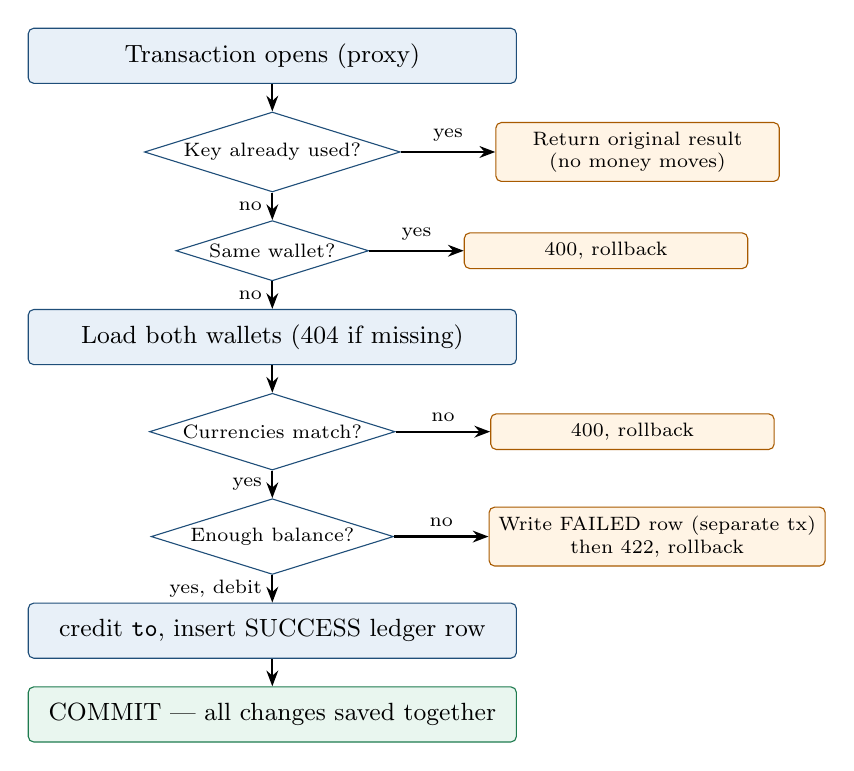
\begin{tikzpicture}[
  node distance=0.35cm,
  stp/.style={draw=brand,fill=brandlight,rounded corners=2pt,minimum width=6.2cm,minimum height=0.7cm,align=center,font=\small},
  dec/.style={draw=brand,fill=white,diamond,aspect=3.2,inner sep=1pt,align=center,font=\scriptsize},
  bad/.style={draw=warnorange,fill=warnbg,rounded corners=2pt,align=center,font=\scriptsize,minimum width=3.6cm},
  good/.style={draw=okgreen,fill=okbg,rounded corners=2pt,align=center,font=\small,minimum width=6.2cm,minimum height=0.7cm},
  arr/.style={-{Stealth[length=2mm]},thick}]
\node[stp] (start) {Transaction opens (proxy)};
\node[dec,below=of start] (key) {Key already used?};
\node[dec,below=of key] (same) {Same wallet?};
\node[stp,below=of same] (load) {Load both wallets (404 if missing)};
\node[dec,below=of load] (cur) {Currencies match?};
\node[dec,below=of cur] (bal) {Enough balance?};
\node[stp,below=of bal] (move) {credit \code{to}, insert SUCCESS ledger row};
\node[good,below=of move] (commit) {COMMIT --- all changes saved together};
\node[bad,right=1.2cm of key] (k1) {Return original result\\(no money moves)};
\node[bad,right=1.2cm of same] (s1) {400, rollback};
\node[bad,right=1.2cm of cur] (c1) {400, rollback};
\node[bad,right=1.2cm of bal] (b1) {Write FAILED row (separate tx)\\ then 422, rollback};
\draw[arr] (start)--(key); \draw[arr] (key)--node[left,font=\scriptsize]{no}(same);
\draw[arr] (same)--node[left,font=\scriptsize]{no}(load); \draw[arr] (load)--(cur);
\draw[arr] (cur)--node[left,font=\scriptsize]{yes}(bal); \draw[arr] (bal)--node[left,font=\scriptsize]{yes, debit}(move);
\draw[arr] (move)--(commit);
\draw[arr] (key)--node[above,font=\scriptsize]{yes}(k1); \draw[arr] (same)--node[above,font=\scriptsize]{yes}(s1);
\draw[arr] (cur)--node[above,font=\scriptsize]{no}(c1); \draw[arr] (bal)--node[above,font=\scriptsize]{no}(b1);
\end{tikzpicture}
\end{center}

\begin{itemize}
  \item \textbf{Cheap checks first.} The same-wallet check needs no database, so it runs before loading anything
        (our unit test verifies the repository is never touched in that case).
  \item \textbf{Everything in one transaction.} If the ledger insert failed after the debit, the debit is undone too.
        Money can never vanish or be created.
  \item \textbf{Currency check.} Sending 100 INR into a USD wallet as ``100 USD'' would create money out of thin air.
\end{itemize}

\subsection{Idempotency: never send money twice}
\label{sec:idem}
\begin{simplebox}[The problem]
You tap ``Pay'' and your internet drops. Did the payment go through? The app doesn't know, so it
retries. Without protection, the server might process \emph{both} requests: you pay twice.
\end{simplebox}

\textbf{The solution:} the client generates a unique ID (a UUID) per payment attempt and sends it in the
\code{Idempotency-Key} header. Retries reuse the same key. The server stores the key with the ledger row:
\begin{itemize}
  \item first request with key \code{K}: transfer happens, row saved with \code{idempotency_key = K};
  \item retry with key \code{K}: the lookup finds the existing row and returns it. \textbf{No second transfer.}
\end{itemize}
Postman request 7 proved this: same key, same transaction id returned, Alice charged once (749.50).

\textbf{What if two identical requests arrive at the exact same moment?} Both may pass the lookup.
But the \code{UNIQUE} constraint on \code{idempotency_key} means only one \code{INSERT} can succeed. The other
transaction fails at commit and \textbf{rolls back entirely, including its debit}. So money still moves once.
(In Phase 1 the loser gets a 409; Phase 3 will make it return the original result instead.)

\begin{interviewbox}
``Idempotent means doing it twice has the same effect as doing it once. The check-then-act lookup is the
fast path; the unique constraint is the real guarantee, because only the database can arbitrate a race
between two concurrent requests.''
\end{interviewbox}

\subsection{\code{FailedTransferRecorder} and \code{REQUIRES\_NEW}}
\begin{lstlisting}
@Component
public class FailedTransferRecorder {
    @Transactional(propagation = Propagation.REQUIRES_NEW)
    public void record(Long fromWalletId, Long toWalletId, BigDecimal amount,
                       String idempotencyKey, String reason) {
        transactionRepository.save(Transaction.failedTransfer(
                walletRepository.getReferenceById(fromWalletId),
                walletRepository.getReferenceById(toWalletId),
                amount, idempotencyKey, reason));
    }
}
\end{lstlisting}

\textbf{What:} when a transfer fails for insufficient balance, we still want a \code{FAILED} row in the
ledger (useful for auditing and fraud detection).

\textbf{The trap:} the transfer's transaction is about to roll back. If we inserted the FAILED row inside
it, the rollback would delete that row too. Nothing would be recorded.

\textbf{The fix:} \code{Propagation.REQUIRES_NEW} tells Spring to \emph{pause} the current transaction,
start a brand-new independent one, commit it, then resume the original (which then rolls back). The
FAILED row survives.

\textbf{Why a separate class?} Remember the proxy: \code{@Transactional} only works when the call goes
\emph{through} the proxy. If \code{TransferService} called its own \code{this.record()}, the call would
skip the proxy (``self-invocation''), \code{REQUIRES_NEW} would be ignored, and the row would be rolled back.
Putting it in another bean forces the call through a proxy.

\textbf{\code{getReferenceById}} returns a lightweight placeholder holding only the id. That's all we need
to fill in the foreign keys, so no extra \code{SELECT} runs.

\begin{interviewbox}
This is one of the best questions to steer an interview toward: ``How do you log a failure
when the transaction that failed rolls back?'' Answer: \code{REQUIRES_NEW} in a separate bean, and
explain self-invocation. It shows you understand how Spring works inside, not just how to use it.
\end{interviewbox}

\subsection{Concurrency and optimistic locking}
\label{sec:optimistic}
\textbf{The danger (``lost update'' / double spending):} Alice has 100. Two transfers of 80 arrive at the
same time on two threads.

\begin{center}
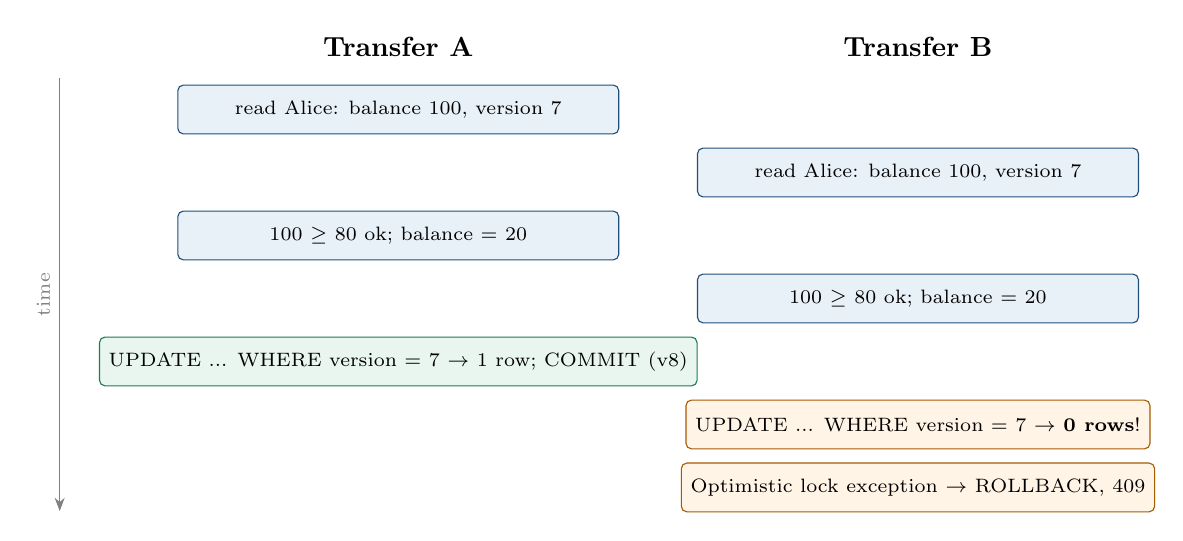
\begin{tikzpicture}[font=\small,
  ev/.style={draw=brand,fill=brandlight,rounded corners=2pt,minimum width=5.6cm,minimum height=0.62cm,align=center,font=\scriptsize},
  evbad/.style={draw=warnorange,fill=warnbg,rounded corners=2pt,minimum width=5.6cm,minimum height=0.62cm,align=center,font=\scriptsize},
  evok/.style={draw=okgreen,fill=okbg,rounded corners=2pt,minimum width=5.6cm,minimum height=0.62cm,align=center,font=\scriptsize}]
\node[font=\bfseries] at (0,0) {Transfer A};
\node[font=\bfseries] at (6.6,0) {Transfer B};
\node[ev] at (0,-0.8) {read Alice: balance 100, version 7};
\node[ev] at (6.6,-1.6) {read Alice: balance 100, version 7};
\node[ev] at (0,-2.4) {100 $\geq$ 80 ok; balance = 20};
\node[ev] at (6.6,-3.2) {100 $\geq$ 80 ok; balance = 20};
\node[evok] at (0,-4.0) {UPDATE ... WHERE version = 7 $\rightarrow$ 1 row; COMMIT (v8)};
\node[evbad] at (6.6,-4.8) {UPDATE ... WHERE version = 7 $\rightarrow$ \textbf{0 rows}!};
\node[evbad] at (6.6,-5.6) {Optimistic lock exception $\rightarrow$ ROLLBACK, 409};
\draw[-{Stealth},gray] (-4.3,-0.4) -- node[left,rotate=90,anchor=south,font=\scriptsize]{time} (-4.3,-5.9);
\end{tikzpicture}
\end{center}

Without \code{@Version}, B's update would simply overwrite A's: Alice ends with 20 but 160 was sent.
That's \textbf{80 rupees created from nothing}. With \code{@Version}, B's stale update matches no rows, so
it fails safely. Alice ends at 20, only 80 was sent, and the books balance.

\begin{center}
\begin{tabularx}{\textwidth}{>{\bfseries}l X X}
\toprule
 & Optimistic locking (what we use) & Pessimistic locking (alternative) \\
\midrule
Idea & Don't lock; detect conflicts at write time with a version number. & Lock the row when reading (\code{SELECT ... FOR UPDATE}); others wait. \\
Good when & Conflicts are rare (most transfers touch different wallets). & Conflicts are frequent (one very hot account). \\
Cost & Loser must retry. & Waiting, and risk of deadlocks if locks are taken in different orders. \\
\bottomrule
\end{tabularx}
\end{center}

In Phase 1 the losing request gets \textbf{409 Conflict} (``please retry''). Phase 3 adds automatic retries
\emph{outside} the transaction, and Phase 4 proves it with a test firing 10 concurrent transfers.

% =====================================================================
\section{Controllers: The REST Endpoints}
% =====================================================================

\subsection{The endpoints}
\begin{center}
\begin{tabularx}{\textwidth}{l >{\ttfamily}l X l}
\toprule
Method & \normalfont\bfseries Path & What it does & Success \\
\midrule
POST & /api/auth/register & Create a user (password hashed) & 201 \\
POST & /api/wallets & Create a wallet for a user & 201 + \code{Location} \\
GET  & /api/wallets/\{id\} & Get a wallet and its balance & 200 \\
POST & /api/wallets/\{id\}/deposit & Add money to a wallet & 200 \\
POST & /api/transfers & Send money between wallets & 201 \\
\bottomrule
\end{tabularx}
\end{center}

\subsection{How a controller looks}
\begin{lstlisting}
@RestController
@RequestMapping("/api/wallets")
@RequiredArgsConstructor
public class WalletController {
    private final WalletService walletService;

    @PostMapping
    public ResponseEntity<WalletResponse> create(@Valid @RequestBody CreateWalletRequest request) {
        WalletResponse wallet = walletService.create(request);
        URI location = ServletUriComponentsBuilder.fromCurrentRequest()
                .path("/{id}").buildAndExpand(wallet.id()).toUri();
        return ResponseEntity.created(location).body(wallet);
    }
    ...
}
\end{lstlisting}

\begin{itemize}
  \item \code{@RestController} = this class handles HTTP and its return values become JSON.
  \item \code{@RequiredArgsConstructor} (Lombok) generates a constructor for the \code{final} fields;
        Spring uses it to \textbf{inject} the service (\emph{constructor injection}, the recommended style:
        dependencies are explicit and the class is easy to test).
  \item \code{@RequestBody} = read the JSON body; \code{@PathVariable} = read \code{\{id\}} from the URL;
        \code{@RequestHeader} = read a header (the idempotency key).
  \item Creating something returns \textbf{201 Created} plus a \code{Location} header pointing to the new
        resource, which is standard REST practice.
\end{itemize}

\begin{whybox}[Why are controllers so thin?]
Controllers only translate HTTP to Java and back. All rules live in services, so the same logic could
be reused from a message queue or a scheduled job, and tested without starting a web server.
\end{whybox}

\textbf{Temporary shortcut:} \code{CreateWalletRequest} contains a \code{userId}, so anyone could create a
wallet for anyone. That's acceptable only because Phase 1 has no login. In Phase 2 the owner will come from
the JWT token, and \code{userId} will be removed from the request.

% =====================================================================
\section{Error Handling}
% =====================================================================

\subsection{Custom exceptions}
\begin{lstlisting}
public abstract class BusinessException extends RuntimeException {
    private final HttpStatus status;
    protected BusinessException(HttpStatus status, String message) { ... }
}
public class WalletNotFoundException extends BusinessException {
    public WalletNotFoundException(Long id) {
        super(HttpStatus.NOT_FOUND, "Wallet " + id + " not found");
    }
}
\end{lstlisting}

\begin{center}
\begin{tabularx}{\textwidth}{>{\ttfamily}l l X}
\toprule
\normalfont\bfseries Exception & \bfseries HTTP & \bfseries When \\
\midrule
WalletNotFoundException & 404 & Wallet id doesn't exist \\
UserNotFoundException & 404 & User id doesn't exist (creating a wallet) \\
InsufficientBalanceException & 422 & Not enough money \\
InvalidOperationException & 400 & Same-wallet transfer, currency mismatch, bad amount, bad idempotency key \\
EmailAlreadyExistsException & 409 & Email already registered \\
\bottomrule
\end{tabularx}
\end{center}

\textbf{Why a base class that carries the status?} The global handler needs only \emph{one} method for all
business errors. Adding a new error type later means writing one small class, not touching the handler.

\textbf{Why 422 for insufficient balance?} The request is perfectly valid JSON (so not 400); the server
understood it but can't carry it out given the current state. 422 ``Unprocessable Content'' says exactly that.

\subsection{\code{GlobalExceptionHandler}}
A class annotated \code{@RestControllerAdvice} catches exceptions thrown by any controller and turns them
into the same JSON shape:

\begin{lstlisting}[style=plain]
{
  "timestamp": "2026-11-01T12:30:05Z",
  "status": 422,
  "error": "Unprocessable Content",
  "message": "Insufficient balance in wallet 1: available 749.5000, requested 999999",
  "path": "/api/transfers"
}
\end{lstlisting}

\begin{center}
\begin{tabularx}{\textwidth}{>{\ttfamily\footnotesize\raggedright\arraybackslash}p{6.6cm} l X}
\toprule
\normalfont\bfseries Caught & \bfseries HTTP & \bfseries Why \\
\midrule
BusinessException (all subclasses) & own & Our expected errors \\
MethodArgumentNotValidException & 400 & \code{@Valid} failed; response lists \code{fieldErrors} \\
HttpMessageNotReadableException & 400 & Broken JSON \\
MethodArgumentTypeMismatchException & 400 & e.g.\ \code{/api/wallets/abc} \\
ObjectOptimisticLockingFailureException & 409 & \code{@Version} conflict --- safe to retry \\
DataIntegrityViolationException & 409 & A unique constraint fired (race) \\
Exception (anything else) & 500 & Logged on the server; client sees only ``Unexpected error'' \\
\bottomrule
\end{tabularx}
\end{center}

\begin{whybox}
\textbf{Consistency:} clients need one parser for all errors. \textbf{Security:} stack traces reveal
class names, library versions and SQL, all useful to attackers. Unknown errors are logged in full on
the server but the client only sees a generic message.
\end{whybox}

% =====================================================================
\section{Security in Phase 1}
% =====================================================================

Adding the Spring Security dependency \emph{locks every endpoint by default} (it generates a random
password and demands login). Since login only arrives in Phase 2, \code{SecurityConfig} temporarily opens
everything:

\begin{lstlisting}
@Bean
public SecurityFilterChain securityFilterChain(HttpSecurity http) throws Exception {
    http.csrf(AbstractHttpConfigurer::disable)
        .sessionManagement(s -> s.sessionCreationPolicy(SessionCreationPolicy.STATELESS))
        .authorizeHttpRequests(auth -> auth.anyRequest().permitAll());
    return http.build();
}

@Bean
public PasswordEncoder passwordEncoder() { return new BCryptPasswordEncoder(); }
\end{lstlisting}

\begin{itemize}
  \item \textbf{CSRF disabled:} CSRF attacks abuse \emph{cookies} that browsers send automatically. Our API will
        use tokens in the \code{Authorization} header, which browsers never attach on their own, so CSRF
        protection isn't needed.
  \item \textbf{STATELESS:} the server keeps no login session in memory; every request must prove who it is
        (with a JWT in Phase 2). This lets you run many server copies behind a load balancer.
  \item \textbf{PasswordEncoder bean:} one shared BCrypt hasher, injected into \code{UserService}.
\end{itemize}

\begin{warnbox}[Phase 1 is NOT secure yet --- on purpose]
Right now anyone can read any wallet or move money from any wallet. That's acceptable only on your
laptop while building. Phase 2 fixes it with JWT authentication and ownership checks, and the app
will not be deployed publicly before that.
\end{warnbox}

% =====================================================================
\section{Testing}
% =====================================================================

\subsection{Unit tests (11 tests, all passing)}
A \textbf{unit test} checks one class in isolation, in milliseconds, without a database or web server.

\subsubsection*{\code{WalletTest} (5 tests): the money rules}
\begin{itemize}
  \item \code{creditThenDebitUpdatesBalance} --- 100.50 $-$ 40.25 = 60.25 exactly.
  \item \code{decimalAmountsStayExact} --- 0.1 + 0.2 = 0.3 (would fail with \code{double}).
  \item \code{debitMoreThanBalanceIsRejectedAndBalanceUnchanged} --- even 0.0001 too much is rejected and nothing changes.
  \item \code{debitOfExactBalanceLeavesZero} --- spending everything is allowed.
  \item \code{zeroOrNegativeAmountsAreRejected}.
\end{itemize}

\subsubsection*{\code{TransferServiceTest} (6 tests): the transfer logic with Mockito}
\textbf{Mockito} creates fake versions (\emph{mocks}) of the repositories. We tell them what to return
(``when \code{findById(1)} is called, return Alice's wallet'') and later \emph{verify} what was called. This
tests the service's logic alone, with no MySQL needed.

\begin{lstlisting}
@Test
void insufficientBalanceRecordsFailedRowAndChangesNothing() {
    stubWallets(alice, bob);                       // alice has 100
    assertThatThrownBy(() -> transferService.transfer(
            new TransferRequest(1L, 2L, new BigDecimal("100.01")), "key-2"))
        .isInstanceOf(InsufficientBalanceException.class);

    assertThat(alice.getBalance()).isEqualByComparingTo("100");   // unchanged
    verify(failedTransferRecorder).record(eq(1L), eq(2L), eq(new BigDecimal("100.01")),
                                          eq("key-2"), anyString());
    verify(transactionRepository, never()).save(any());          // no SUCCESS row
}
\end{lstlisting}

The six cases: successful transfer; insufficient balance (FAILED row recorded, nothing else);
same-wallet rejected before touching the DB; unknown wallet $\rightarrow$ 404; currency mismatch;
repeated idempotency key returns the original without moving money.

Tests follow the \textbf{Arrange--Act--Assert} pattern: set up data, call the method, check the result.
Run them with:
\begin{lstlisting}[style=plain]
.\mvnw.cmd test
\end{lstlisting}
(The generated \code{FincoreApplicationTests.contextLoads} starts the whole app, so it needs MySQL
running and your \code{.env} in place.)

\subsection{End-to-end testing with Postman (16/16 checks)}
Unit tests use fakes; Postman tests the \emph{real} running app against the \emph{real} database. The
collection \code{postman/FinCore-Phase1.postman_collection.json} runs 12 requests in order. Each request
saves the ids the next ones need (e.g.\ Alice's wallet id) using small test scripts.

\begin{center}
\begin{tabularx}{\textwidth}{>{\raggedright\arraybackslash}p{5.2cm} l X}
\toprule
Request & Result & What it proves \\
\midrule
1--2 Register Alice, Bob & 201 & Users created, passwords hashed \\
3--4 Create wallets & 201 & Wallets start at 0 \\
5 Deposit 1000 & 200 & Balance exactly 1000; DEPOSIT ledger row \\
6 Transfer 250.50 & 201 & SUCCESS, both balances updated in one transaction \\
7 Replay same key & 201 & Same transaction id: \textbf{no double payment} \\
8 Check Alice & 200 & 749.50: debited exactly once \\
9 Transfer 999999 & 422 & Insufficient balance, FAILED row recorded \\
10 Same wallet & 400 & Business rule enforced \\
11 Amount $-50$ & 400 & Validation, with \code{fieldErrors.amount} \\
12 Wallet 999999 & 404 & Clean not-found error \\
\bottomrule
\end{tabularx}
\end{center}

The red 4xx badges in Postman are \emph{expected}: those requests were designed to fail, and the tests
check that they fail correctly.

\subsection{Checking the database directly}
\begin{lstlisting}[style=plain]
SELECT id, balance, version FROM fincore.wallets;
SELECT id, type, status, amount, failure_reason FROM fincore.transactions;
\end{lstlisting}
You should see the \code{version} column increase each time a wallet changes, and a ledger with one
DEPOSIT, one SUCCESS TRANSFER and one FAILED TRANSFER per collection run.

% =====================================================================
\section{Git and the Project History}
% =====================================================================

\subsection{What we did}
\begin{enumerate}
  \item Your GitHub repo \code{piyush-nfx/fincore} was empty. Your CryptoVault code was in a separate local
        repo (\code{Desktop/Projects/cryovault}, remote \code{piyush-nfx/CryptoVault}) with 3 commits.
  \item In the FinCore folder: \code{git init -b main} and added the GitHub remote.
  \item Imported CryptoVault's history without touching the original folder:
\begin{lstlisting}[style=plain]
git fetch ../../cryovault main      # copy its commits into this repo
git reset --soft FETCH_HEAD         # point main at them, keep FinCore files staged
git tag -a v1-cli -m "CryptoVault v1 ..." FETCH_HEAD
\end{lstlisting}
  \item Committed FinCore on top. That commit adds the 45 Spring Boot files and removes the 16 old CLI files
        from \code{main}; the tag still holds them.
  \item Verified the password was not in any staged file, then pushed \code{main} and the tag.
\end{enumerate}

\begin{lstlisting}[style=plain]
8d0a2bd (main)   FinCore v2: rebuild CryptoVault as a Spring Boot wallet REST API (Phase 1)
5536a58 (v1-cli) Feature: Added interactive CLI menu loop using Scanner
571c587          Initial commit: Complete OOP Crypto Wallet Simulation
784f0dc          Initial commit: Core OOP wallet architecture with history and file logging
\end{lstlisting}

\begin{whybox}[Why keep the old history?]
It tells your growth story in the repo itself: v1 CLI $\rightarrow$ v2 REST API. An interviewer can run
\code{git checkout v1-cli} to see where you started. A \textbf{tag} is a permanent bookmark on a commit, ideal
for marking a version.
\end{whybox}

\subsection{A small bug found in the old repo}
CryptoVault's ignore file was named \code{.gitignore.txt}. Git only reads a file named exactly
\code{.gitignore}, so it was ignored and IntelliJ's \code{.idea} files got committed. FinCore has a proper
\code{.gitignore} (which also excludes \code{target/} and \code{.env}).

\subsection{Other practical notes}
\begin{itemize}
  \item The project lives inside \textbf{OneDrive}. Sync can lock files during builds. If you see strange
        ``file in use'' errors, move the project to a non-synced folder like \code{D:\textbackslash Projects}.
  \item The commit message includes a \code{Co-Authored-By} line because the code was written with an AI
        assistant. Be ready to explain every line yourself; this document is meant to help with exactly that.
\end{itemize}

% =====================================================================
\section{Known Limitations (Planned Fixes)}
% =====================================================================

Being honest about limitations is a strength in interviews. These are deliberate for Phase 1:

\begin{center}
\begin{tabularx}{\textwidth}{>{\raggedright\arraybackslash}p{6cm} X l}
\toprule
Limitation & Fix & Phase \\
\midrule
No login: anyone can read or move anyone's money & JWT authentication + ownership checks & 2 \\
\code{userId} sent in the create-wallet body & Owner taken from the token & 2 \\
Optimistic-lock conflict returns 409; client must retry & Automatic retry (up to 3) outside the transaction & 3 \\
\code{Idempotency-Key} is optional & Make it required for transfers & 3 \\
Keys are unique globally, not per user & Scope keys to the user & 3 \\
Same-key race: loser gets 409 & Catch the conflict and return the original result & 3 \\
Replaying a FAILED key still answers 201 & Return the matching status code & 3 \\
No transaction history endpoint & \code{GET /api/transactions?page=0&size=10} & 3 \\
No concurrency proof yet & 10-thread double-spend test & 4 \\
\bottomrule
\end{tabularx}
\end{center}

% =====================================================================
\section{Interview Questions You Can Now Answer}
% =====================================================================

\newcommand{\qa}[2]{\textbf{Q: #1}\par\vspace{-2pt}#2\par\vspace{6pt}}

\qa{Why did you rebuild CryptoVault?}{An \code{ArrayList} plus a text file can't handle concurrent users,
isn't crash-safe, and has no authentication. I moved to Spring Boot + MySQL to get ACID transactions,
optimistic locking, and (Phase 2) JWT security.}

\qa{Why BigDecimal for money?}{\code{double} is binary floating point and can't represent 0.1 exactly
(0.1 + 0.2 = 0.30000000000000004). \code{BigDecimal} is exact decimal arithmetic; the column is
\code{DECIMAL(19,4)}. And compare with \code{compareTo}, not \code{equals}.}

\qa{How do you make sure a transfer is all-or-nothing?}{Debit, credit and the ledger insert run in one
\code{@Transactional} method. Spring's proxy commits if the method returns and rolls back on any
\code{RuntimeException}, so a partial transfer can never be saved.}

\qa{What happens if two transfers hit the same wallet at once?}{Both read version $n$. The first commits
and bumps it to $n+1$. The second's \code{UPDATE ... WHERE version = n} matches zero rows, Hibernate throws an
optimistic-locking exception, the transaction rolls back, and the client gets 409. No lost update, no double
spend.}

\qa{Optimistic vs pessimistic locking?}{Optimistic detects conflicts at commit time (cheap when conflicts
are rare; loser retries). Pessimistic locks rows with \code{SELECT ... FOR UPDATE} (others wait; better for hot
rows; risk of deadlocks). Most transfers touch different wallets, so optimistic fits.}

\qa{What is idempotency and how did you implement it?}{Repeating a request has the same effect as sending it
once. Clients send an \code{Idempotency-Key}; if we've seen it, we return the stored result. A \code{UNIQUE}
constraint on the column guarantees it even when two copies race.}

\qa{How do you record a failed transfer if the transaction rolls back?}{A separate bean with
\code{@Transactional(propagation = REQUIRES_NEW)} commits the FAILED row in its own transaction. It must be a
separate bean because self-invocation bypasses Spring's proxy.}

\qa{Why DTOs instead of returning entities?}{To avoid leaking fields like the password hash, to decouple the
API from the database schema, to prevent lazy-loading surprises and infinite JSON loops, and to block mass
assignment.}

\qa{Why is the ledger immutable?}{Auditability. Like a bank statement, past entries are never edited; a
correction is a new entry. Every balance can be recomputed from the ledger.}

\qa{Why BCrypt?}{It's one-way, salted per password, and deliberately slow, so stolen hashes are expensive to
crack. It only uses the first 72 bytes, so we cap password length at 72.}

\qa{What does \code{open-in-view=false} do?}{It closes the persistence context when the service transaction
ends, so no hidden lazy-loading queries run while JSON is being written, and DB connections are held for less
time.}

\qa{What is dirty checking?}{Hibernate tracks entities loaded in a transaction and, at commit, automatically
issues \code{UPDATE}s for whatever changed. That's why deposit doesn't call \code{save(wallet)}.}

\qa{How did you keep secrets out of GitHub?}{Config reads \code{${DB_PASSWORD}}; real values live in a
git-ignored \code{.env} (imported via \code{spring.config.import}) locally, and in environment variables on the server.
A committed \code{.env.example} documents the names.}

% =====================================================================
\section{Glossary}
% =====================================================================

\begin{description}[leftmargin=3.6cm,style=nextline,itemsep=3pt]
  \item[REST API] A way for programs to talk over HTTP using URLs (\code{/api/wallets/1}) and verbs (GET, POST).
  \item[JSON] Text format for data: \code{\{"amount": 250.50\}}.
  \item[Spring Boot] Framework that wires your Java app together and runs an embedded web server.
  \item[Bean] An object Spring creates and manages (services, repositories, controllers).
  \item[Dependency injection] Spring hands a class the objects it needs (via the constructor) instead of the class creating them.
  \item[JPA / Hibernate] JPA is the standard for mapping objects to tables; Hibernate is the implementation that writes the SQL.
  \item[Entity] A Java class mapped to a table.
  \item[DTO] A plain class/record describing API input or output.
  \item[Transaction] A group of DB operations that succeed or fail together.
  \item[ACID] Atomicity, Consistency, Isolation, Durability.
  \item[Proxy] A wrapper object Spring puts around a bean to add behaviour (like transactions) before/after method calls.
  \item[Optimistic locking] Detect concurrent edits using a version number instead of locking.
  \item[Idempotency] Doing something twice has the same effect as doing it once.
  \item[Ledger] Append-only list of every money movement.
  \item[BCrypt] Slow, salted, one-way password hashing algorithm.
  \item[Mock] A fake object used in tests to stand in for a real dependency.
  \item[HTTP status] 2xx success, 4xx client mistake, 5xx server failure.
  \item[JWT] JSON Web Token, a signed token proving who you are (Phase 2).
  \item[Git tag] A permanent named bookmark on a commit (e.g.\ \code{v1-cli}).
\end{description}

\vspace{1em}
\begin{tcolorbox}[colback=okbg,colframe=okgreen,arc=2pt]
\textbf{Next: Phase 2 --- Security.} Login with JWT access and refresh tokens, a filter that verifies the
token on every request, ``you can only use your own wallets'' (preventing IDOR), and an ADMIN-only
endpoint.
\end{tcolorbox}

\end{document}
